\chapter{The fourth protocol - Removing The Overhead}
\label{chap:fourthProtocol}

% **************************** Define Graphics Path **************************
\ifpdf
    \graphicspath{{Chapter7/Figs/Raster/}{Chapter7/Figs/PDF/}{Chapter7/Figs/}}
\else
    \graphicspath{{Chapter7/Figs/Vector/}{Chapter7/Figs/}}
\fi

% ***** Main ****

\section{Introduction}
\label{sec:6intro}
In the last chapter, we developed the two-parties authentication protocol that
is secure against malicious client and does not leak any information to the
server (the main difference with the second protocol is the server learns the
value of the distance only). The final variant aims to reduce both communication
size and computation time of the third variant while providing all the security
features.
\begin{description}
\item[Reducing Communication Size] We observe that the main bottle neck of the
  communication is the size of the Stern-based ZKPs. We propose the
  following approach to replace the old ZKPs
  \begin{itemize}
  \item A Schnorr-based approach to replace the Stern-based one, to prove the
    noise in the ciphertext is small. This variant reduces the total
    communication rounds from \(log_{2/3}(FAR)\) to only 1.
  \item A challenge-response protocol to prove the binary format of the
    plaintext. The protocol can be summarized as follows
    \begin{enumerate}
    \item The server samples \(r_{1}, r_{2} \randomsample R_{q}\) and computes
      \(ch = enc(r_{1}*Q*(1-Q) + r_{2}) + enc(0,r)\) and sends \(ch\) to the
      client.
    \item The client decrypts the result and sends back \(rsp\).
    \item The server accepts the response if and only if \(rsp = r_{2} \)
    \end{enumerate}
    We remark that the first operation needs to be computed bit-wise, that means
    we need to change the ciphertext packing method, the CRT-packing
    \cite{smart2014fully} can support this requirement.
  \end{itemize}
\item[Reducing Computation Time.] With the application of new ciphertext packing
  method, we can effectively change the way of computing Hamming Distance by
  summing the bits of the XOR result of 2 bitstring instead of computing the
  inner product. Therefore, with this approach we save the computation by doing
  addition only without any homomorphic multiplication. The cost of this change
  is a set of switching keys for homomorphic rotation operations, which are
  generated during enrollment process. Additionally, we introduce the
  appplication of state-of-the-art \textit{Secure-Multiparty-Protocol}
  techniques such as \textit{Garbled Circuit} and \textit{Oblivious Transfer} in
  the lattice-based context to further improve both of the computation time and
  the communication size overhead from previous ZKP protocols.
\end{description}
This approach is practical because it moves a major part of the overhead to the
one-time set up phase of the protocol (the enrollment stage). Our result shows
that the protocol can work efficiently during authentication stage. The
technique maybe generalized to similar multi-stages protocols.

\section{The Challenge-Response Technique}
\label{sec:6challenge}
Consider this situation.  Alice sends a ciphertext \(C\) of a bitstring to
Bob. Bob is supposed to use homomorphic encryption technique to process
\(C\). Before doing so, Bob might want to make sure that \(C\) is an encryption
of a bitstring and not something else. How can he do that? Suppose that the
plaintext \(P\) is encoded as coefficients of a polynomial, or specifically,
\(P\) can be an element of the ring \(R_{2}\), where
\(R_{2} = \frac{\mathbb{Z}_{2}[x]}{x^{n} + 1}\), this ring is used by many RLWE
based cryptosystems lately. One solution can be applying Zero Knowlege Proof
technique. This is however a costly solution. There are mainly two approaches
for ZKP, the Schnorr's based protocol, e.g. \cite{benhamouda2014better} or
Stern's based protocol such as \cite{stern1993new} or
\cite{ling2013improved}. The first approach has limitation on the norm of the
secret it can prove and cannot be used to prove the knowledge of binary message
with norm 2. The second approach can prove binary but it has very high
communication cost due to roundness error of \(2/3\).

\section{The BGV Cryptosystem and CRT packing method}
\label{sec:6bgv}
\paragraph{Ciphertext packing}

We have seen that a plaintext can be packed in a specific way to support the
homomorphic operations efficiently. The approach of \cite{yasuda2014practical}
can help the inner product operations perform really fast, however, it does not
support Single Instruction Multiple Data (SIMD) operation, which is required by
our challenge-response protocol. This section discuss another approach for
plaintext packing and the operations that it supports: the CRT packing method
\cite{smart2014fully}. In this method, a message \(\mathbf{m} \in R_{t}\) is
packed by represent it in the NTT domain. In NTT domain, a single operation
(addition or multiplication) of a pair of ciphertexts implicitly computed
component-wise the entire plaintext vectors. Beside SIMD support, we can also
\textit{rotate} or \textit{permute} the plaintext slots
(\cite{gentry2012fully}), we will need only \textit{rotate} operation in this
project.

\paragraph{Number Theoretic Transform}
In our application context, the most costly low level computation operation is
the ring multiplication (polynomial multiplication). This section discusses the
Number Theoretic Transform (NTT), the technique providing efficient algorithms
for cyclic and nega-cyclic convolutions that can be applied to compute
polynomial multiplication efficiently. Moreover, in our research context, when
the message is represented in the NTT domain, the operations are computed
component wise simultaneously, this important property help our
challenge-response protcol to save the most communication size compared with
ZKPs overhead of the previous protocols.
\begin{description}
\item[Notations] Given \(a(x) = a_{0} + a_{1}x + \dots + a_{n-1}x^{n-1}\) and
  \(b(x) = b_{0} + b_{1}x + \dots + b_{n-1}x^{n-1}\), we denote \(\cdot\) to be
  the convolution multiplication and \(\triangle\) to be the component wise
  multiplication of the two polynomials.
\item[Introduction] One of the most important applications of Fast Fourier
  Transform (FFT) is multiplication of large integers and polynomial
  multiplication (which is the cyclic convolution of two integer sequences). The
  later operation can be computed by applying the FFT to the sequences, then
  multiplying the result component wise and applying the inverse FFT to the
  product:
  \[
    a(x)\cdot b(x) = FFT^{-1}(FFT(a(x)) \triangle FFT(b(x)))
  \]
  When the coefficients are elements of a finite field, the FFT is called the
  Number Theoretic Transform (NTT). We recall the definition of NTT: Given the
  parameters of our context, with \(n\) is a power of 2 and \(t\) is a prime
  with \(t = 1 \mod 2n\), let
  \(\mathbf{a} = [a_{0}, a_{1}, \dots, a_{n-1}] \in R_{t}\) and let \(\omega\)
  be a primitive \(n^{th}\) root of unity in \(\mathbb{Z}_{t}\), that is,
  \(\omega^{n} = 1 \mod t\). The forward transform
  \(NTT(\mathbf{a}) = \tilde{\mathbf{a}}\) is defined as
  \(\tilde{\mathbf{a}}_{i} = \sum_{j=0}^{n-1}{\mathbf{a}_{j}}\omega^{ij} \mod
  t\) for \(i = 0, \dots, n -1\). Informally, the coefficients of
  \(\tilde{\mathbf{a}}\) are the evaluations of the polynomial \(a(x)\) at the n
  roots of unity. The inverse transformation is given by
  \(\mathbf{b} = NTT^{-1}(\tilde{\mathbf{a}})\), where
  \(\mathbf{b}_{i} = n^{-1}\sum_{j=0}^{n-1}\tilde{\mathbf{a}}_{j}\omega^{-ij}
  \mod t \) for \(i = 0, \dots, n - 1\). We have
  \(NTT^{-1}(NTT(\mathbf{a})) = \mathbf{a}\).  The above convolution operation
  computes a polynomial \(c(x) = a(x)\cdot b(x)\) with order at most \(2n - 1\),
  therefore in normal polynomial multiplication scenarios, \(a(x)\) and \(b(x)\)
  are padded with coefficients 0 before applying NTT. If the original \(a(x)\)
  and \(b(x)\) are not padded with 0s, the result product corresponds to the
  actual product modulo \(x^{n} - 1\).
  \[
a(x) \cdot b(x) \mod (x^{n} - 1) = NTT^{-1}(NTT(a(x)) \triangle NTT(b(x)))
  \]

  However, in our contexts, we want the operations are computed modulo
  \(x^{n} + 1\), one can still pad the original ring elements with 0s and
  compute the product modulo \(x^{n} + 1\), this will double the length of NTT
  inputs and also require an extra step of explicite reducing \(x^{n} + 1\). The
  other way to avoid this issue is by exploiting the \textit{negative wrapped
    convolution} \cite{lyubashevsky2008swifft}. Let \(\psi\) be a primitive
  \(2n^{th}\) root of unity in \(\mathbb{Z}_{t}\) such that
  \(\psi^{2} = \omega\) and denote \(NTT_{+}(\mathbf{a})\) to be the special NTT
  transform such that
  \(NTT_{+}(\mathbf{a}) = NTT(\mathbf{a} \triangle (1, \psi, \psi^{2}, \dots,
  \psi^{n-1}))\) and
  \(NTT_{+}^{-1}(\mathbf{a}) = NTT^{-1}(\mathbf{a}) \triangle (1, \psi^{-1},
  \psi^{-2}, \dots, \psi^{-(n-1)})\). It can be proved that
  \(NTT_{+}(\mathbf{a})\) is the evaluations of \(a(x)\) at the odd roots of the
  \(2n^{th}\) roots of unity:
  \(NTT_{+}(\mathbf{a}) = (a(\omega_{0}), a(\omega_{1}), \dots,
  a(\omega_{n-1}))\), where \(\omega_{i} = \psi^{2i + 1}\). It turns out that
  \[
a(x) \cdot b(x) \mod (x^{n} + 1) = NTT_{+}^{-1}(NTT_{+}(a(x)) \triangle NTT_{+}(b(x)))
  \]
  Since most of our works are based on
  \(R_{q} = \frac{\mathbb{Z}_{q}}{x^{n} + 1}\), when we mention NTT throughout
  the text, we imply the operation is done with \(NTT_{+}\) instead of normal
  NTT. In the implementation, in order to find \(\psi\), we need to find the
  group element such that \(\psi^{2} = \omega \mod t\), where \(\omega\) is the
  \(n^{th}\) root of unity. There are heuristic approaches to find the square
  root of an element, in our context, we can find it easily (the problem is
  finding an element with order of \(2n\)). Given \(n, t\) such that
  \(2n | (t - 1)\) (these parameters are set up at the initialization stage of
  the protocol), if we can find a generator \(g\) of order \(t -1\) in
  \(\mathbb{Z}_t^{*J}\), then \(\psi = g^{\frac{t-1}{2n}}\):
\[
  order(g^{\frac{t-1}{2n}}) = \frac{t-1}{gcd(\frac{t-1}{2n},t-1)} =
  \frac{t-1}{(\frac{t-1}{2n})} = 2n
\]

\end{description}






\subsection{The rotate and permute function}
\label{sec:6rotate}

\paragraph{Slot Rotation}

Given a polynomial
\(a(x) = (a_{0}, a_{1}, \dots, a_{n-1}) \in \mathbb{Z}_{t}^{n}\), let
\(\mathbf{a}\) be the coefficient representation of \(a(x)\) and
\(\hat{\mathbf{a}}\) be the NTT representation of \(a(x)\). The \textit{rotate}
operation is a mapping \(K\) such as
\(a(x) \stackrel{K_{j}}{\mapsto} a(x^{j})\), where \(j\) is the number of
positions being rotated and \(gcd(j,n) = 1\). This operation can be done on
either the coefficient or the NTT representation of \(a(x)\).
\begin{description}
\item[Coefficients domain] In order to map
  \(a(x) \stackrel{K_{j}}{\mapsto} a(x^{j})\), or
  \[\mathbf{a} = (a_{0}, a_{1}, \dots, a_{n-1}) \stackrel{K_{j}}{\mapsto} a(x^{j}) = a_{0} + a_{1}(x^{j})^{1} + a_{2}(x^{j})^{2} + \dots + a_{n-1}(x^{j})^{n-1}\]
  We can look at the relation between the coefficients before and after the
  mapping: Each of the mapped result coefficient \(a_{i}(x^{j(n-i)})\) will be
  mapped to one of the original position \(a_{l}\) for \(l = 0,\dots,n-1\) when
  we do modulo \(x^{n} + 1\), or \(x^{n} = -1\). In other word, the rotate
  operation of \(\mathbf{a}\) is just a permutation of the original coefficients
  with some sign changes on some coefficients. However, we are more interested
  in the rotation operation in the NTT domain as our message was packed with CRT
  packing method.
\item[NTT domain] Given \(\mathbf{\hat{a}}\), which is the evaluation of
  \(a(x)\) at the n primitive \(2n^{th}\) roots of unity modulo \(t\) (Section
  \ref{sec:6bgv}):
  % \[
  %   \mathbf{\hat{a}} = (\hat{a}_{0}, \hat{a}_{1}, \dots, \hat{a}_{n-1}) =
  %   (a(\omega_0), a(\omega_1), \dots,
  %   a(\omega_{n-1})) \text{, where } \omega_i = \psi_{2n}^{2i+1}
  % \]
  The rotate operation maps \(\mathbf{\hat{a}}\) to
  \(\mathbf{\hat{b}} = (\hat{b}_{0}, \hat{b}_{1}, \dots, \hat{b}_{n-1})\), where
  \(\hat{b}_{i} = a(x^{j})|_{x = \omega_{i}} = a(\omega_{i}^{j}) =
  a(\psi^{(2i+1)j})\). We can see that the rotation on the NTT domain is also a
  permution of the original coefficients, the difference compared to the
  operation on coefficient domain is that it does not have the sign change
  effect on the original coefficients. However, this permutation is not the one
  we need for the HD computation algorithm (Algorithm \ref{alg:hd-comp-homom}):
  the \(i^{th}\) CRT component of \(\mathbf{\hat{a}}\) is the \(i'^{th}\) CRT
  component of \(\mathbf{\hat{b}}\), where \(i'\) satisfies
  \(2i' +1 \equiv (2i + 1)j \mod 2n\).

  We define \(\mathbf{\bar{a}}\) to be also the evaluation of \(a(x)\) at the
  \(n\) primitive \(2n^{th}\) roots of unity modulo \(t\), but in a different
  order, such that when applying the rotation operation, we will get back
  exactly the order we need for the HD computation algorithm. The idea is, with
  \(n\) a power of 2, those 2n-th roots of unity
  \(\mathbf{\psi_{i}} \textnormal{ for } i = 0, \dots, n-1\) form a group that
  is isomorphic to the multiplicative group of integers modulo n (the set of
  congruence classes relatively prime to the modulo n), denoted by
  \(\mathbb{Z}_{2n}^{*}\). Note that this group \(\mathbb{Z}_{2n}^{*}\) is not a cyclic group but it can
  be generated by sets of ``generators''. For \(n\) is a power of 2, the group
  \(\mathbb{Z}_{2n}^{*}\) can be generated by
  \((3)^{x}(-1)^{y} \textnormal{ for } x \in \mathbb{Z}_{n/2} \textnormal{ and } y
  \in \mathbb{Z}_{2}\). The polynomial \(\mathbf{\bar{a}}\) can be represented by

  \begin{align*}
       \mathbf{\bar{a}} = (a(\psi^{3^{0}(-1)^{0}}),a(\psi^{3^{1}(-1)^{0}}), \dots,
    a(\psi^{3^{n/2 -1}(-1)^{0}}), \\ a(\psi^{3^{0}(-1)^{1}}),
    a(\psi^{3^{1}(-1)^{1}}), \dots,a(\psi^{3^{n/2 -1}(-1)^{1}}))
  \end{align*}

  Each coefficient of \(\mathbf{\bar{a}}\) can be indexed and denoted as follows
  \[
    \bar{a}_{i,i'} = a(\psi^{3^{i}(-1)^{i'}}) \textnormal{ for } i \in
    \mathbb{Z}_{n/2} \textnormal{ and } i' \in \mathbb{Z}_{2}
  \]

  Let's look at the mapping \(a(x) \stackrel{K_{j}}{\mapsto} a(x^{j})\) again under this new
  representation. Denote \(b(x) = a(x^{j})\), where
  \(j \in \mathbb{Z}_{2n}^{*}\). We remark that every value of \(j\) can also be
  represented by
  \(j = 3^{x_{j}}(-1)^{y_{j}}, (x_{j} \in \mathbb{Z}_{n/2} \textnormal{ and }
  y_{j} \in \mathbb{Z}_{2})\). We have
  \begin{align*}
    \mathbf{\bar{b}} = (b(\psi^{3^{0}(-1)^{0}}),b(\psi^{3^{1}(-1)^{0}}), \dots,
    b(\psi^{3^{n/2 -1}(-1)^{0}}), \\ b(\psi^{3^{0}(-1)^{1}}),
    b(\psi^{3^{1}(-1)^{1}}), \dots,b(\psi^{3^{n/2 -1}(-1)^{1}}))\\
    = (a((\psi^{3^{0}(-1)^{0}})^{3^{x_{j}}(-1)^{y_{j}}}),a((\psi^{3^{1}(-1)^{0}})^{3^{x_{j}}(-1)^{y_{j}}}), \dots,
    a((\psi^{3^{n/2 -1}(-1)^{0}})^{3^{x_{j}}(-1)^{y_{j}}}), \\ a((\psi^{3^{0}(-1)^{1}})^{3^{x_{j}}(-1)^{y_{j}}}),
    a((\psi^{3^{1}(-1)^{1}})^{3^{x_{j}}(-1)^{y_{j}}}), \dots,a((\psi^{3^{n/2 -1}(-1)^{1}})^{3^{x_{j}}(-1)^{y_{j}}}))\\
    = (a(\psi^{3^{0 + x_{j}}(-1)^{0 + y_{j}}}), a(\psi^{3^{1 + x_{j}}(-1)^{0 + y_{j}}}), \dots,a(\psi^{3^{n/2 - 1 + x_{j}}(-1)^{0 + y_{j}}}),\\
    a(\psi^{3^{0 + x_{j}}(-1)^{1 + y_{j}}}), a(\psi^{3^{1 + x_{j}}(-1)^{1 + y_{j}}}), \dots, a(\psi^{3^{n/2 - 1 + x_{j}}(-1)^{1 + y_{j}}}))
  \end{align*}

  By this representation, we see that the \(\mathbf{\bar{b}}\)'s coefficients
  \(\bar{b}_{i,i'}\) are the \(\mathbf{\bar{a}}\)'s coefficients
  \(\bar{a}_{i+x_{j} \mod n/2, i' + y_{j} \mod 2}\). In effect we will have a
  rotation here! It is not exactly a normal rotation, but it is 2 rotations on
  the 2 halves, each of the half rotates by \(x_{j}\) position and they will
  swap if \(y_{j} = 1\). In our context, we can take
  \(x_{j} = 2^{0}, 2^{1}, \dots, 2^{\log n/2}\) and \(y_{j} = 0\) to add up the
  bits of each half, then we swap the halves by setting \(x_{j} = 0\) and
  \(y_{j} = 1\) to add up all the bits to get the final value of Hamming
  Distance.
  
  For ciphertexts that are the multiplication or addition of polynomials, when
  we map their rotations, we can perform each individual rotation and then do
  the original operation:
\begin{align*}
  a(x).b(x) \mapsto a(x^{j}).b(x^{j})\\
  a(x) + b(x) \mapsto a(x^{j}) + b(x^{j})
\end{align*}

Therefore, a ciphertext of the form
\(c = (\mathbf{as} + t \mathbf{e} + \mathbf{m}, -\mathbf{a})\) can be rotated by
doing the mapping on each of the components \(\mathbf{a},\mathbf{s},\mathbf{e}\)
and \(\mathbf{m}\) before adding up the results.
\end{description}

\subsection{The flattening gadget}
\label{sec:6flattening}

\subsection{The keyswitch and modswitch operation}
\label{sec:6keyswitch}

\section{HD computation}
\label{sec:6hdcomp}

\section{Garbled Circuit and Oblivious Transfer}
\label{sec:6garbled}

\subsection{Oblivious Transfer}
In 1-out-of-2 Oblivious Transfer protocol (denoted by
\(\begin{psmallmatrix} 2 \\ 1 \end{psmallmatrix} \)-OT), a \textit{sender} has
two choices \(m_{0}, m_{1}\), and a \textit{receiver} has one bit \(b\) as its
input. At the end of the protocol, the \(receiver\) learns \(m_{b}\) and the
sender learns nothing about the \(receiver\)'s query.

\subsection{Yao Garbled Circuit}
\label{sec:yao-garbled-circuit}

% \graphicspath{{Chapter7/Figs/Vector/}}
% \begin{center}
% \input{Chapter7/Figs/Vector/GC.pdf_tex}
% \end{center}

The concept of garbled circuit was proposed in \missref{``yao generate exchange
  secret''}, it allows 2 parties to evaluate securely any function (represented
as boolean circuits). We refer to the \(server\) as the one who prepares the
circuit and the \(client\) is the one evaluating the circuit. The general idea
is that given a function composed of logic gates that are connected by wires,
the server ``garbles'' the circuit by assigning two random cryptographic keys
\(K_{j}^{0}\) and \(K_{j}^{1}\) to each wire \(j\). The keys represent 0 and 1
values, which are the possible inputs to each wire, in related literature, keys
are also referred to as \textit{labels.}  The server then encrypts a truth table
for each gate of the circuit such that in order to compute the \textit{output
  label } of a gate, one must know the \textit{labels}, or keys of the input,
this is achieved by double encryption using possible combinations of the input
keys. Figure \missref{} shows an example of a simple gate with its key and truth
table.

The final output of the function is also represented as pair of keys, the server
knows the value of the function output corresponding to each
\textit{label}. After setting up the garbled circuit, the server sends it to the
client and its input's keys. The client then uses OT technique discussed to
obtain the keys corresponding to its inputs. During evaluating the circuit, the
client decrypt one \textit{label} \(K_{j}^{i}\) for each output wire \(j\),
where \(i \in \{0,1\}\) and use the decrypted result to continue evaluating the
circuit until it get the final keys of the circuit. The client then sends the
final labels to the server to verify the function's output.

Recent improvements reduce both computation time and communication overhead
associated with circuit setup and evaluation. \missref{``vsedvenka 30''}
described a technique that allow XOR gates to be evaluated \textit{for free}:
there is no communication overhead with such gates and the evaluation does not
involve cryptographic operations. \missref{``vsedvenka 38''} proposed a
mechanism to reduce the communication size of binary gates by 25\%: each gate
can be specified by encoding only three outcomes instead of all four. The
research by \missref{``vsedvenka 29''} improved the complexity of basic
operations (addition, multiplication, comparison, etc) by reducing the number of
non-XOR gates.



\section{The details}
\label{sec:4thProcDetails}

\subsection{The protocol description}
\label{sec:4thprocSteps}
    
\begin{figure}[h!]
  \centering
    \begin{equation*}
        \begin{array}{c c c}
        \text{\textbf{Client}} & & \text{\textbf{Server}} \\
          \\
          \text{1. Registered template \textbf{T}} & \xrightarrow{\enc{\mathbf{T}}} & \text{Store } \enc{\mathbf{T}}\\
          
          \text{2. Query template \textbf{Q}} & \xrightarrow{\enc{\mathbf{Q}}} & \text{Initiate Query Proof}\\

                               & \xleftrightarrow{\text{3. Prove small noise in \textbf{Q}}} & \\

                               & \xleftrightarrow{\text{4. Prove \textbf{Q} is binary}} & \\

                               & & \text{Sample \(r \randomsample \mathbb{Z}_{t}\)}\\
                               & & \text{5. Setup garbled circuit GC, for } i = 1,\dots,k \\

                               & & \text{6. Setup } (K^{0}_{r_{i}}, K^{1}_{r_{i}}) \text{ for } GC_r \\
          
                               & & \text{7. Setup } (K^{0}_{h_{i}}, K^{1}_{h_{i}}) \text{ for } GC_{h}\\
          
                               & & \text{8. Setup } (K^{0}_{out}, K^{1}_{out}) \\

                               & & \text{9. Compute } \enc{K^0_{h_i}},\enc{K^1_{h_i}}\\
          \\

                               & & \text{10. } \enc{\mathbf{HD}} = HDBGV(\enc{\mathbf{T}},\enc{\mathbf{Q}}) \\
          
                                   & & \text{Compute } \enc{\mathbf{HD'}} = \enc{\mathbf{HD + r}}\\

                               & \xleftarrow{\enc{\mathbf{HD'}}} & \\

                               & \xleftarrow{GC} & \\

                               & \xleftarrow{K_{r_i}^j \text{of } GC_r} & \\

          \text{12. Decrypt } \mathbf{HD'} = dec(\enc{\mathbf{HD}}) & & \\

          \text{13. Decompose } \mathbf{HD'} = \sum_{i=0}^k{2^ih_i} & & \\

          \text{14. Encrypt } \enc{h_i} & & \\
          
          \text{15. Initiate OT protocol} & & \\

                               & \xrightarrow{16. \enc{h_i}} & \\
          
                               & \xrightarrow{\text{17. Prove correct decryption}} & \\

                               & \xleftarrow{\text{18. Retrieve } \enc{K_{h_i}^j}} & \\

          \text{19. Decrypt } K_{h_i}^j & & \\
          20. K_{out} = GC( K_{h_i}^j , K_{r_i}^j) & & \\

                               & \xrightarrow{K_{out}} & \text{21. Compare } K_{out} \text{ with } K_{out}^0, K_{out}^1 \\
          & & \text{ Output res = \textbf{Accept|Reject}}
        \end{array}
    \end{equation*}

  \caption{The fourth protocol}
  \label{fig:fourthProtocol}
\end{figure}

\subsection{The Garble Circuit and Oblivious Transfer}
We use standard substractor circuit for the operation \(HD = HD' - r\). Given 2
n-bit bitstring, the circuit is built from 1 half-substractor and \(n-1\)
full-substractors as in Figure \ref{fig:substractor}

\begin{figure}[htbp!] 
  \centering    
  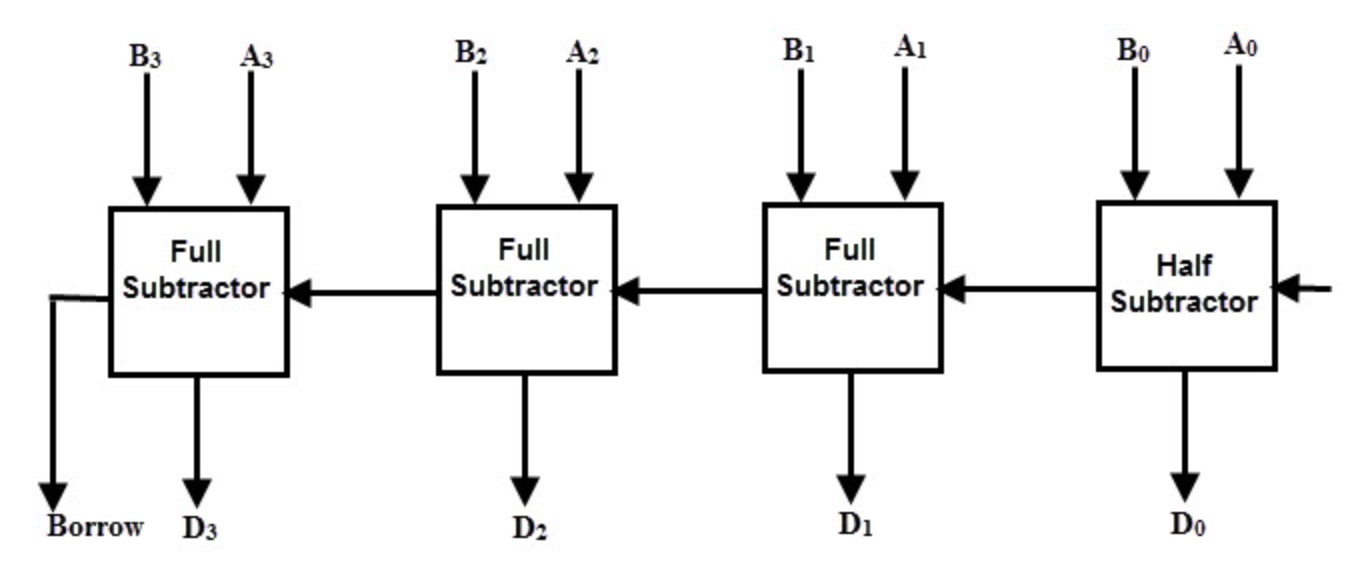
\includegraphics[width=1.0\textwidth]{Chapter7/Figs/Raster/subCircuit}
  \caption{Substractor Circuit}
  \label{fig:substractor}
\end{figure}

Where a half-substractor is built from 1 XOR gate and 1 AND gate, a full-substractor is built from 2 half-substractors and 1 OR gate (Figure \ref{fig:fullSubstractor})

\begin{figure}[htbp!] 
  \centering    
  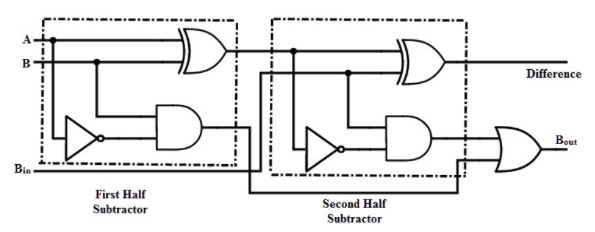
\includegraphics[width=1.0\textwidth]{Chapter7/Figs/Raster/fullSubstractor}
  \caption{Half-substractor and Full-substractor}
  \label{fig:fullSubstractor}
\end{figure}

For our context, let \(l\) to be the bit length of the HD' and r (\(l\) is
typically 10-12 bits for 1024-2048 bits biometrics data), so we need about
\(5l\) gates for the substractor logic gates. The comparision circuit needs not
to output 3 result as standard ones (where they can output either A > B, A < B
or A = B), we simply want to check whether \(HD' - r < \tau\), so we can simply
have another l NAND gates plus \(l-1\) XOR gates for the comparsion circuit (An
example is as in Figure \ref{fig:comparisionCircuit})

\begin{figure}[htbp!] 
  \centering    
  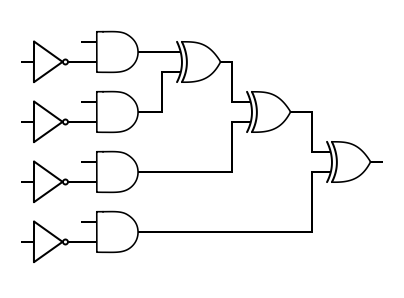
\includegraphics[width=1.0\textwidth]{Chapter7/Figs/Raster/comparisionCircuit}
  \caption{Comparator Circuit}
  \label{fig:comparisionCircuit}
\end{figure}

\paragraph{Garble Circuit preparation}
We denote \(GC\) to be the garbled circuit prepared by the server. The inputs to
the circuit include the server's \(GC_{r}\) and the client's \(GC_{h}\), which
are the cryptographic key \textit{labels} corresponding to the server's input
\(r\) and client's input \(HD'\) to the function \textit{CompareHD}. The main
function of the circuit is, it first substracts \(HD' - r = HD\) then compares
\(HD \stackrel{?}{<} \tau\), where \(\tau\) is the constant value of the
threshold to decide the authentication result, which can be built into the
circuit itself. We note that either the server or the client can do the role of
setting up the garbled circuit, in our work, we let the server take this role
(Figure \ref{fig:fourthProtocol} - Step 5, 6, 7, 8) for the reason that we have
been working on \textit{semi-honest} server modeal and \textit{malicious }
client, this will save us one proof to prove that the circuit is generated
correctly.

As described before in Section \ref{sec:yao-garbled-circuit}, the server garbles
the circuit \(GC\) and sends to the client together with its \textit{labels} of
\(r\), which are \(K_{r_{i}}^{j}\). Next, the client uses our OT technique
(\missref{}) to select the correct \textit{labels} of \(HD'\): the first part of
the OT will ensure that the client will get back the encryptions
\(\enc{K_{h_{i}}^{j}}\). The second part of the OT makes sure that the protocol
is secure against \textit{malicious} clients: it needs to prove that it
decrypted and decompose \(\enc{\mathbf{HD'}}\) correctly (Figure
\ref{fig:fourthProtocol} - Step 12,13). In other words, the client wants to
prove that the encryptions \(\enc{h_{i}}\) that he sent is actually the
encryption of the bits of \(HD'_{i}\). Recall that the server still has
\(\enc{\mathbf{HD'}}\), so the proof can be a homomorphically check of
\(\enc{\mathbf{HD'}} - \sum{2^{i}\enc{h_{i}}} = \enc{0}\). This proof is part of
the proof we did in the third variant of the protocol \missref{}. However, in
order to do this proof to support the homomorphic operations, we need to use the
same encryption scheme for the OT protocol, in other words, we need an OT
protocol based on BGV.

We note that inside the garbled circuit, AES is normally used to encrypt the
\textit{labels}, this encryption is a part of the garbled circuit and not
related to the OT protocol we just described and can still be used independently
to ensure the performance of circuit evaluations. Next, we discuss an approach
to design an OT protocol that is compatible with BGV cryptosystem

\paragraph{BGV-based OT}
\todo{review PVW08, oblivious transfer LWE}

This section describes a technique to use BGV homomorphic operations to
implement an OT protocol. The technique can be used together with the garbled
circuit protocol discussed earlier. The problem can be stated as follows: Given
a BGV ciphertext of a bit selection \(h_{i}\): \(\enc{h_{i}}\), the server
computes and returns a BGV encryption of the corresponding key selected by the
bit. We observe that the following homomorphic operations will obtain such
requirement:
\[
\enc{K_{i}^{j}} = \enc{h_{i}^{j}} \cdot \enc{K_{i}^{1}} + (1 - \enc{h_{i}^{j}}) \cdot \enc{K_{i}^{0}}
\]
Where \(K_{i}^{0}, K_{i}^{1}\) are the \textit{labels} corresponding to the wire
inputs 0 or 1. The function include one level of homomorphic multiplication, two
additions and one multiplication with a constant. This approach is simple enough
and it is secure against \textit{malicious client} model in our context because
the client had to do the proof that he actually encrypted \(\enc{h_{i}}\)
correctly already. Other applications of this OT should take into account that a
malicious client can encrypt \(\enc{h_{i}}\) incorrectly to learn about
\(K_{i}^{0}\) and/or \(K_{i}^{1}\).

The other issue that we have to be careful about is \textit{Circuit Privacy}:
for a multi-factor attacker that has access to the secret key but not the
biometric template, it can learn about information of the randomness of the
operation. The randomness of the above operation is of the form
\(K_{i}^{0} + (K_{i}^{1} - K_{i}^{0})r_{0}\), which is correlated to both of the
keys. Again, we can mask the randomness of this leakage similarly to what we did
in the second variant of the protocol. By similar analysis, we can still show
that computing the HD cannot be done with significant probability (the privacy
security requirement is relaxed from what the client sees is indistinguishable
to the probability that he can compute the HD is not much more than random
guessing). This will be detailed in the security analysis \missref{}.






\subsection{HD Computation Homomorphically - BGV}
Given two bistring \(\mathbf{a}\) and \(\mathbf{b}\) of length \(n\) (for \(n\)
is a power of 2), the Hamming Distance \(HD_{(\mathbf{a,b})}\) can be computed
by adding up and rotating all the bits of \(\mathbf{a} \xor \mathbf{b}\)
(Algorithm \ref{alg:hd-comp-homom}). Provided that the BGV cryptosystem used
supports SIMD operations, the algorithm can run with homomorphic addition and
multiplication. ($\triangle$ denotes component-wise homomorphic multiplication)

\begin{algorithm}
\caption{HD computation}\label{alg:hd-comp-homom}
\begin{algorithmic}[1]
  \Procedure{HDBGV}{$\mathbf{a,b}$}
  \State $\mathbf{c} \gets \mathbf{a} + \mathbf{b} - 2 \mathbf{a} \triangle \mathbf{b}$
  \State let $n \gets length(\mathbf{a})$
  
  \For{$i = 0,\dots,n-1$}
  \State let $\mathbf{t} \gets rotate(\mathbf{c}, 2^{i})$
  \State let $\mathbf{c} \gets add(\mathbf{c}, \mathbf{t})$

  \EndFor
  
\State \textbf{return} $\mathbf{c}[0]$
\EndProcedure
\end{algorithmic}
\end{algorithm}

\section{Results}
\label{sec:6results}


%%% Local Variables:
%%% mode: latex
%%% TeX-master: "../thesis"
%%% End:
